\documentclass[12pt,ngerman]{scrartcl}

\usepackage[T1]{fontenc}
\usepackage{booktabs}
\usepackage{babel}
\usepackage{graphicx}
\usepackage{csquotes}
\usepackage{paralist}
\usepackage{xcolor}
\usepackage{tikz}

\begin{document}


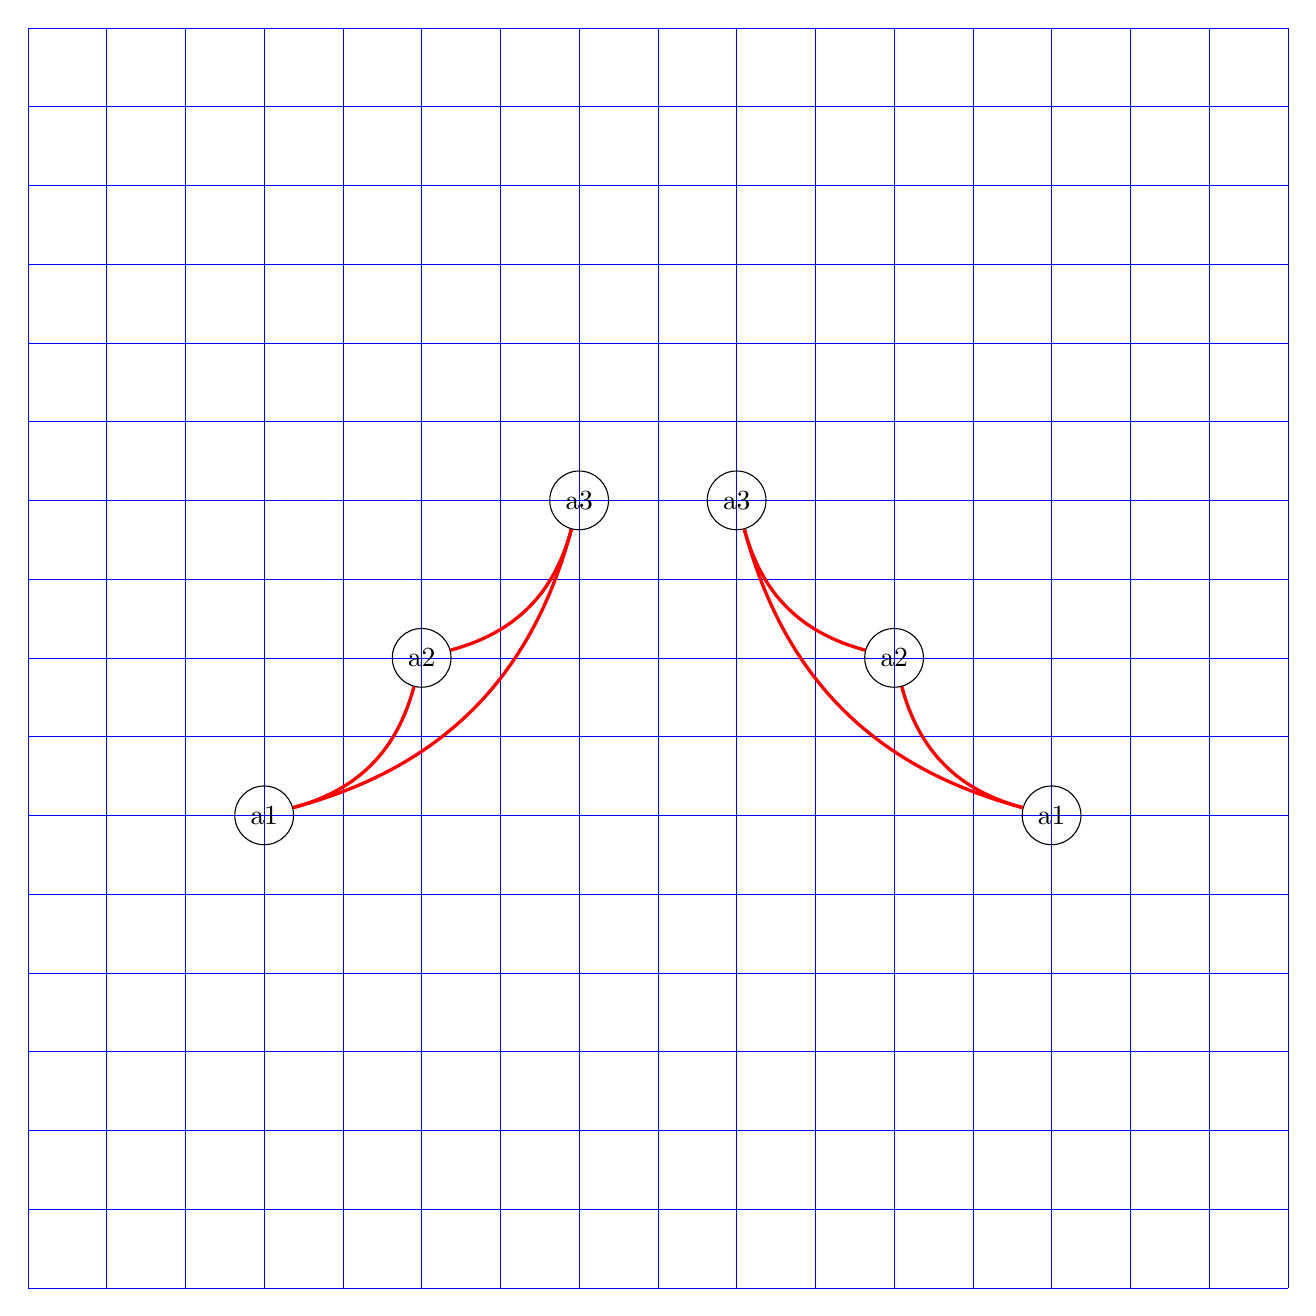
\begin{tikzpicture}
\draw[help lines,blue] (0,0) grid (16,16);

\node[circle,draw,black](a1) at (3,6){a1};
\node[circle,draw,black](a2) at (5,8){a2};
\node[circle,draw,black](a3) at (7,10){a3};

\node[circle,draw,black](b1) at (13,6){a1};
\node[circle,draw,black](b2) at (11,8){a2};
\node[circle,draw,black](b3) at (9,10){a3};

\draw[very thick, red](a1) to [bend right=30] (a3);
\draw[very thick, red](a1) to [bend right=30] (a2);
\draw[very thick, red](a2) to [bend right=30] (a3);

\draw[very thick, red](b1) to [bend right=-30] (b3);
\draw[very thick, red](b1) to [bend right=-30] (b2);
\draw[very thick, red](b2) to [bend right=-30] (b3);

\end{tikzpicture}

\end{document}